%# -*- coding: utf-8-unix -*-
% !TEX program = xelatex
% !TEX root = ../thesis.tex
% !TEX encoding = UTF-8 Unicode
%%==================================================
%% chapter01.tex for SJTU Master Thesis
%%==================================================

%\bibliographystyle{sjtu2}%[此处用于每章都生产参考文献]
\chapter{Introduction}
\label{chap:intro}

% !TEX root = main.tex
% \section{Introduction}
% \label{sec:intro}


Traffic signals coordinate the traffic movements at the intersection and a smart traffic signal control algorithm is the key for transportation efficiency. Traffic signal control has remained as an active research topic because of the high complexity of the problem. The traffic situations are highly dynamic and require the traffic signal plans to be able to adjust to different situations.

Recently, people start to investigate reinforcement learning (RL) techniques for traffic signal control. Recent studies have shown the superior performance of RL technique over traditional transportation approaches~\cite{Wier00,AbPK03,ALUK10,AbMB13,VaOl16,wei2018intellilight}. The biggest advantage of RL is that it directly learns how to take the next actions by observing the feedback from the environment after previous actions. 

\begin{figure}[t!]
\begin{tabular}{ccc}
   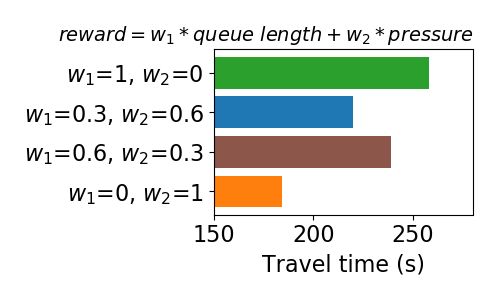
\includegraphics[width=0.24\textwidth]{figures/intro_1.png}&
   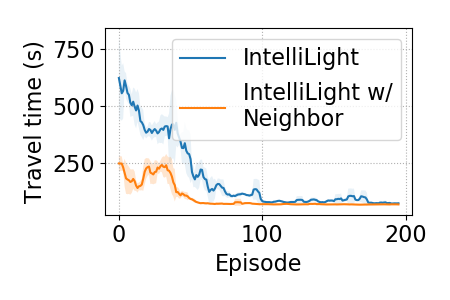
\includegraphics[width=0.215\textwidth]{figures/intro_0.png}\\
   \begin{tabular}[c]{@{}c@{}}(a) Performance w.r.t. reward\end{tabular} &
   \begin{tabular}[c]{@{}c@{}}(a) Convergence w.r.t. state\end{tabular} \\ 
   \end{tabular}
\label{fig:intro}
\caption{Performance of RL approaches is sensitive to reward and state. (a) A heuristic parameter tuning of reward function could result in different performances. (b) The method with a more complicated state (\Deeplight~\cite{wei2018intellilight} w/ neighbor) has a longer learning time but does not necessarily converge to a better result. }
\label{fig:intro}
\vspace{-3mm}
\end{figure}


One most serious issue of current RL-based traffic signal control approaches is that the setting is often heuristic and lacks proper theoretical justification from transportation literature. This often results in highly sensitive performance w.r.t. the setting and leads to long learning process. We elaborate on this issue by examining two fundamental elements in RL setting: reward and state.

First, various reward designs have been proposed. The reason that the reward varies in literature is that travel time, the ultimate objective, is hard to optimize directly. Travel time is a long-term reward after a sequence of actions and the effect of one action can hardly be reflected in terms of travel time. People often choose short-term rewards like queue length or delay to approximate the travel time. So the reward function is often defined as a weighted sum of these terms~\cite{VaOl16,BPT14,ElAb10,ElAA13,wei2018intellilight}. However, as shown in Figure~\ref{fig:intro}(a), tuning the weights on these terms could lead to different results. None of the existing studies has discussed how to define the reward by connecting with the existing transportation method. 

Second, existing RL methods have a trend of using more complicated state representation. Recent studies use visual images to describe the full traffic situation at the intersection~\cite{VaOl16,wei2018intellilight}, which results in the dimension of the state in the scale of thousands. However, as shown in Figure~\ref{fig:intro}(b), complicated state definitions increase the learning time and may not necessarily bring significant gain. Note that we are not claiming that additional information is always not helpful. The choice of the state depends on the reward setting. Based on the reward design of \Deeplight~\cite{wei2018intellilight}, neighboring information is not necessary in the case we shown in Figure~\ref{fig:intro}(a). The question is, could we justify theoretically how much information is enough in state definition in order to optimize the reward function?


\begin{figure}
    \centering
    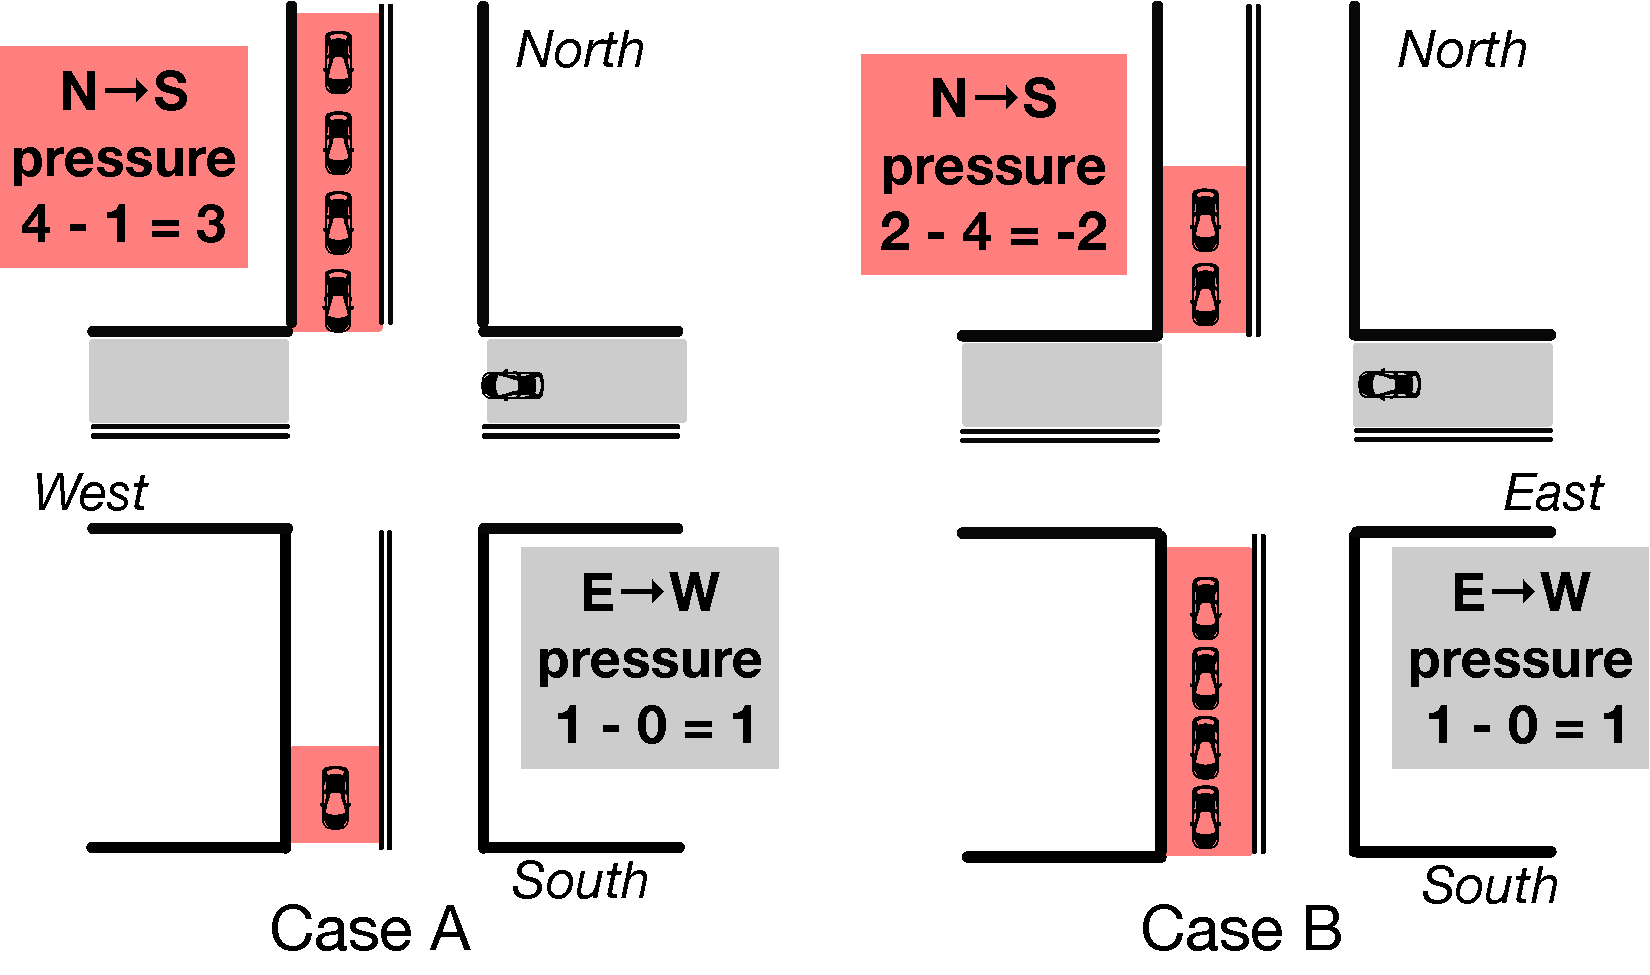
\includegraphics[width=0.3\textwidth]{figures/Maxpressure.pdf}
    \caption{Illustration of max pressure control in two cases. In Case A, green signal is set in the North$\rightarrow$South direction; in Case B, green signal is set in the East$\rightarrow$West direction.}
    \label{fig:pressure}
    \vspace{-2mm}
\end{figure}

The challenges we face in RL motivate us to look for support in transportation approaches. In transportation literature, the state-of-the-art traffic signal control method is max pressure (MP) control~\cite{MP13}. MP has shown to outperform other signal control methods as reported in many recent validation studies~\cite{MP13-adaptvie,MP13}. The key idea of MP is to minimize the ``pressure'' of an intersection., which can be loosely defined as number of vehicles on entering lane minus the number of vehicles on exiting lane. Figure~\ref{fig:pressure} illustrates the concept of pressure. By setting the objective as minimizing the pressure of intersections, MP is proved to maximize the throughput of the whole road network\footnote{Maximizing throughput equals to minimizing travel time under certain conditions and minimizing travel time is the final goal for traffic signal control.}. However, the solution of MP is greedy which leads to locally optimal solutions. 

Our proposed solution is based on RL technique but theoretically grounded by MP method. The connection between RL and MP is that both approaches can essentially be framed as an optimization problem. In RL, reward function is the objective for optimization and the solution is derived from trial-and-error search. In MP, the objective is to minimize pressure and the solution is derived from a greedy algorithm. Intuitively, if we set our reward function the same as the objective of MP, we can achieve the same result as MP. We first prove that under the assumption of no physical queue expansion, both our method and MP are maximizing throughput of the network. We further show that our method can also relax the assumption on physical queue expansion and the conclusion still holds.

To further address the challenge on state design, we describe the system dynamic using the state features based on MP. MP provides evolution equations to formulate the state transition of the traffic as a Markov chain~\cite{MP13book}. In RL, the Markov decision process can formally describe the dynamic of an environment. By including the variables from the evolution equation into state definition in RL, the state is a sufficient statistic for the system dynamic.

We conduct comprehensive experiments using both synthetic data and real data. We test our method in different scenarios of traffic flow and network structure. The evaluation is conducted through traffic simulator. We demonstrate the power of RL methods over traditional transportation approaches because RL optimizes the objective through trial and error. Our method also consistently outperforms state-of-the-art RL methods, which shows that theoretically supported reward design is necessary and the concise design of state leads to efficient learning process.


\nop{

Traffic congestion continues to plague urban environments. Signalized intersections are the most critical bottlenecks for urban arterial networks. Hence, an essential way to mitigate urban traffic congestion is to improve traffic signal control aiming to minimize the average travel time per vehicle. However, multi-intersection traffic signal control is always a complicated problem because the objective of minimizing travel time for all the vehicles cannot be simply divided into minimizing travel time for individual vehicles. Vehicles compete for green signal at an intersection and such competitions are dynamically decided by other traffic signals prior to vehicles' arriving at this intersection. Due to its importance in real world and high complexity of the problem itself, it has drawn interest of researchers in both transportation and computer science fields. 


In transportation research field, there are multiple strategies for traffic signal control. These strategies range from \emph{pre-timed control}, which manually sets the traffic signals based on historical observations of traffic flow patterns~\cite{Mill63}, to \emph{actuated control} which changes traffic signal timings based on current traffic conditions according to some pre-set rules~\cite{CoGD13}, and lastly to \emph{adaptive control}, which dynamically adjusts signal timings according to the real-time traffic data~\cite{}. Among them, adaptive control is the most flexible and responsive approach to dynamic traffic flow. A typical adaptive control solution is based on an \emph{optimization problem formulation}. The high-level objective is to minimize travel time of all vehicles. 

There are two key challenges in optimization-based approaches. First, since the high-level objective (i.e., travel time of all vehicles) is difficult to be optimized directly, the objective is usually simplified. For example, the objective might be optimizing the travel time at individual intersections~\cite{Roess2011t}. Second, various assumptions need to be made in order to make the optimization problem more tractable. There are assumptions regarding the traffic model (e.g., uniform arrival traffic rate~\cite{Webst58}) or road network (e.g., unlimited downstream capacity~\cite{varaiya2013max,MP13-adaptvie, MP13book}). An advantage of such optimization-based approaches is that they have provable theoretical properties in transportation (e.g., maximizing network throughput~\cite{MP13-adaptvie}). However, the assumptions are often very strong and  deviate from  real world conditions, precluding their implementation in real cities. \emph{A central question then becomes, could we have a better method to avoid making such strong assumptions while at the same time keeping the theoretical properties in transportation?}



In computer science research field, researchers are exploring reinforcement learning technique for traffic signal control~\cite{Wier00,AbPK03,ALUK10,AbMB13,VaOl16,wei2018intellilight}. A typical approach is to model each intersection as an agent and the agent optimizes its reward based on the feedback received from the environment after it takes an action. These RL approaches vary in terms of reward design (e.g., queue length~\cite{VaOl16,KWBV08,wei2018intellilight}, delay~\cite{BPT14,ElAb10,ElAA13,VaOl16,wei2018intellilight}), state description (e.g., number of vehicles~\cite{BSSN+05,wei2018intellilight,PraB11}, waiting time~\cite{Wier00,PBTB+13,BPT14}, traffic image~\cite{VaOl16,wei2018intellilight}), learning model (e.g., deep Q-Network~\cite{VaOl16,wei2018intellilight}, policy gradient~\cite{Casa17PG}, actor-critic~\cite{AsMW17AC}), and action design (e.g., setting the phase~\cite{BSSN+05,KWBV08,ALUK10}, change to next phase~\cite{VaOl16,wei2018intellilight,PBTB+13,BPT14}). Some methods further consider coordination among agents by incorporating more neighboring information~\cite{ElAA13,ALUK10,da2006adaptive} or by changing the reward with consideration of neighbors~\cite{VaOl16}. 

\begin{figure}[h]
\begin{tabular}{ccc}
   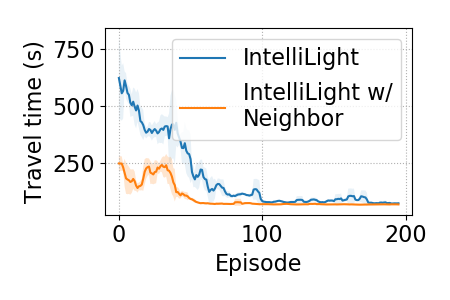
\includegraphics[width=0.215\textwidth]{figures/intro_0.png}&
   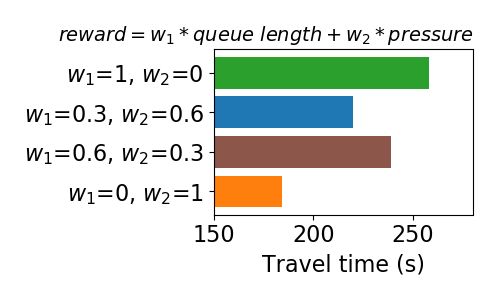
\includegraphics[width=0.24\textwidth]{figures/intro_1.png}\\
   \begin{tabular}[c]{@{}c@{}}(a) Convergence time w/wo \\complicated state\end{tabular} & \begin{tabular}[c]{@{}c@{}}(a) Performance using different \\ weights in reward\end{tabular}\\
   \end{tabular}
\label{fig:intro}
\caption{Performance of RL approaches is sensitive to state and reward. (a) The method with a more complicated state (\Deeplight~\cite{wei2018intellilight} w/ neighbor) has a longer learning time but does not necessarily converge to a better result. (b) A heuristic parameter tuning of reward function could result in different performances.}
\label{fig:intro}
\end{figure}

One serious issue of RL-based traffic signal control approaches is there is no theoretical support for transportation properties, which makes the definition of the RL problem setting heuristic. 
\emph{On one side, existing RL methods have a trend of using more complicated state representation.} Recent studies use visual images to describe the full traffic situation at the intersection~\cite{VaOl16,wei2018intellilight}, which results in the dimension of the state in the scale of thousands. However, as shown in Figure~\ref{fig:intro}(a), more complicated state definitions increase the learning time of the RL algorithm and may not necessarily bring significant gain\footnote{Note that we are not claiming that additional information is always not helpful. The choice of the state depends on the reward setting. Based on the reward design of \Deeplight~\cite{wei2018intellilight}, neighboring information is not necessary in the case we shown in Figure~\ref{fig:intro}(a).}. 
\emph{On the other side, various reward designs have been proposed in literature without proper theoretical justification.} The reason that reward design varies in literature is because travel time, the ultimate objective, is hard to optimize directly. Travel time can be considered as a long-term reward after a sequence of actions, which is a large search space that requires long learning times. So people often choose various features such as queue length and delay to approximate the travel time and the reward function is often a weighted sum of these terms~\cite{VaOl16,BPT14,ElAb10,ElAA13,wei2018intellilight}. However, as shown in Figure~\ref{fig:intro}(b), tuning the weights on these terms could lead to different results and there is no existing study discussing how to set reward in a non-heuristic way. \emph{The question is, could we make our RL approach non-heuristic with the support from transportation theories?}

In the paper, we make an important connection between reinforcement learning and transportation theory by formulating a reinforcement learning problem based on provable transportation theory. In particular, our method is inspired by state-of-the-art max pressure (MP) signal control algorithm~\cite{MP13,MP13book}. The biggest advantage of the MP algorithm is that the objective is proved to maximize throughput of the whole road network system (maximizing throughput equals to minimizing travel time under certain conditions), whereas most existing studies only optimize local transportation efficiency. It has shown to outperform existing traffic signal control methods in transportation field~\cite{MP13,MP13book}. However, the solution of MP is greedy which leads to locally optimal solutions. 

Inspired by MP, we set our reward similar to the objective of MP, which measures the ``pressure'' at the intersection. We first prove that under the assumption of no physical queue expansion, both our RL problem setting and MP are maximizing throughput of the network. We further show that our method can also relax the assumption on physical queue expansion and the conclusion still holds.
Based on the definition of reward, we propose a concise state design and we prove that the state can fully describe the system to optimize the proposed reward. 

We conduct comprehensive experiments using both synthetic data and real data. We test our method in different scenarios of traffic flow and network structure. The evaluation is conducted through traffic simulator. We demonstrate the power of RL methods over traditional transportation approaches because RL optimizes the objective through trial and error instead of making assumptions. Our method also consistently outperforms state-of-the-art RL methods, which shows that theoretically supported reward design is necessary and the concise design of state leads to efficient learning process.
}